% =========================================================================
% figures/rq_tree.tex — Research-questions tree (loads pre-compiled PDF)
% Requires \usepackage{graphicx} in the preamble.
% Insert in the chapter with: % =========================================================================
% figures/rq_tree.tex — Research-questions tree (loads pre-compiled PDF)
% Requires \usepackage{graphicx} in the preamble.
% Insert in the chapter with: % =========================================================================
% figures/rq_tree.tex — Research-questions tree (loads pre-compiled PDF)
% Requires \usepackage{graphicx} in the preamble.
% Insert in the chapter with: % =========================================================================
% figures/rq_tree.tex — Research-questions tree (loads pre-compiled PDF)
% Requires \usepackage{graphicx} in the preamble.
% Insert in the chapter with: \input{figures/rq_tree.tex}
% =========================================================================

\begin{figure}[!ht]
    \centering
    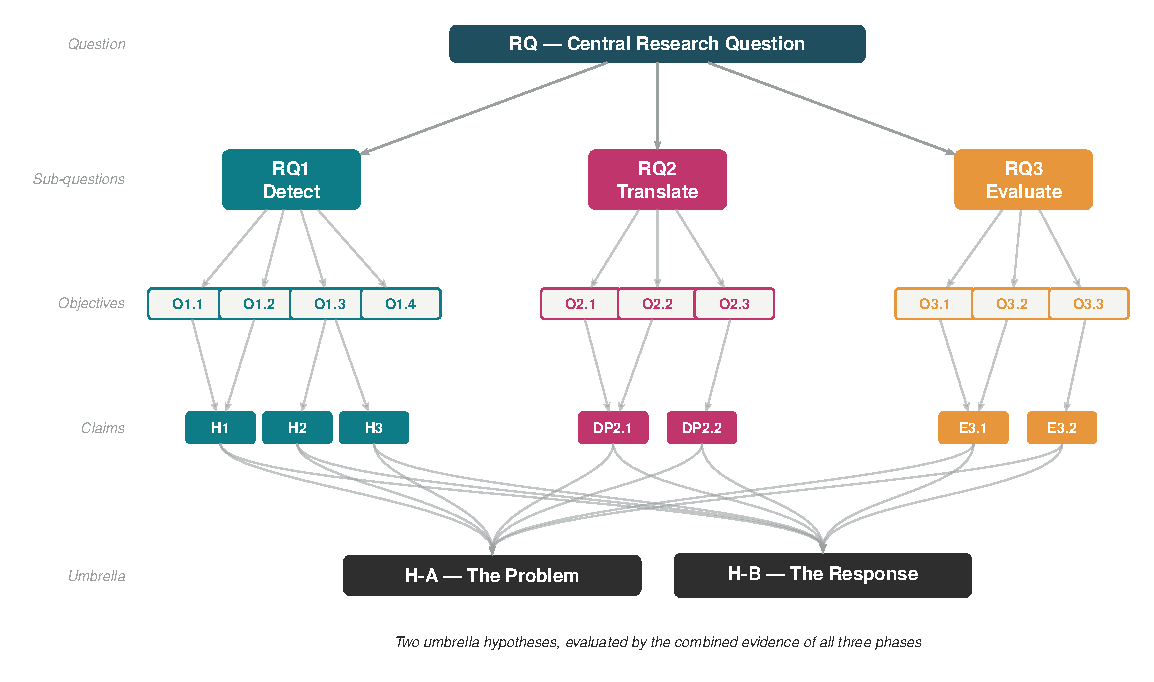
\includegraphics[width=\textwidth]{figures/research_questions/rq_tree_preview.pdf}
    \caption[Structure of the research questions, objectives, claims and umbrella hypotheses.]{\textbf{The
    architecture of the research programme.} The central research question branches into three
    sub-questions along the detect--translate--evaluate arc. Each sub-question generates its objectives
    (O1.1--O1.4, O2.1--O2.3, O3.1--O3.3), which give rise to the claims appropriate to their epistemic
    character: directional hypotheses (H1--H3), design propositions (DP2.1--DP2.2) and empirical
    expectations (E3.1--E3.2). All three claim groups converge on the two umbrella hypotheses, H-A (the
    problem) and H-B (the response), assessed not by any single instrument but by the combined evidence
    of the whole programme.}
    \label{fig:rq-tree}
\end{figure}
% =========================================================================

\begin{figure}[!ht]
    \centering
    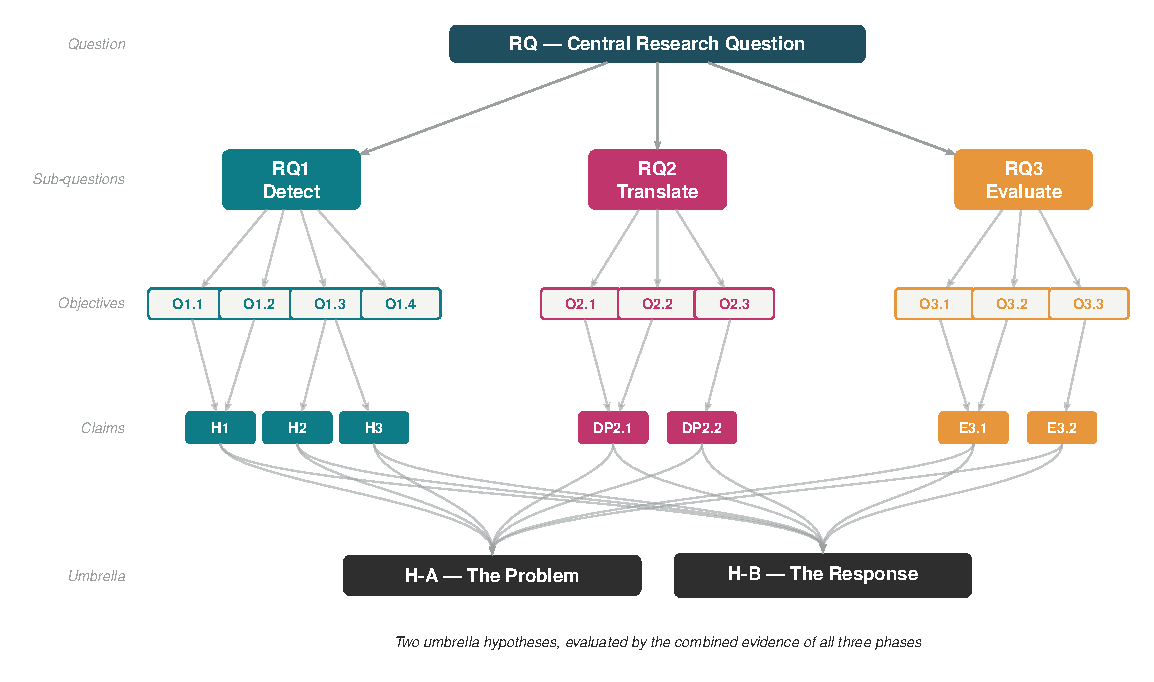
\includegraphics[width=\textwidth]{figures/research_questions/rq_tree_preview.pdf}
    \caption[Structure of the research questions, objectives, claims and umbrella hypotheses.]{\textbf{The
    architecture of the research programme.} The central research question branches into three
    sub-questions along the detect--translate--evaluate arc. Each sub-question generates its objectives
    (O1.1--O1.4, O2.1--O2.3, O3.1--O3.3), which give rise to the claims appropriate to their epistemic
    character: directional hypotheses (H1--H3), design propositions (DP2.1--DP2.2) and empirical
    expectations (E3.1--E3.2). All three claim groups converge on the two umbrella hypotheses, H-A (the
    problem) and H-B (the response), assessed not by any single instrument but by the combined evidence
    of the whole programme.}
    \label{fig:rq-tree}
\end{figure}
% =========================================================================

\begin{figure}[!ht]
    \centering
    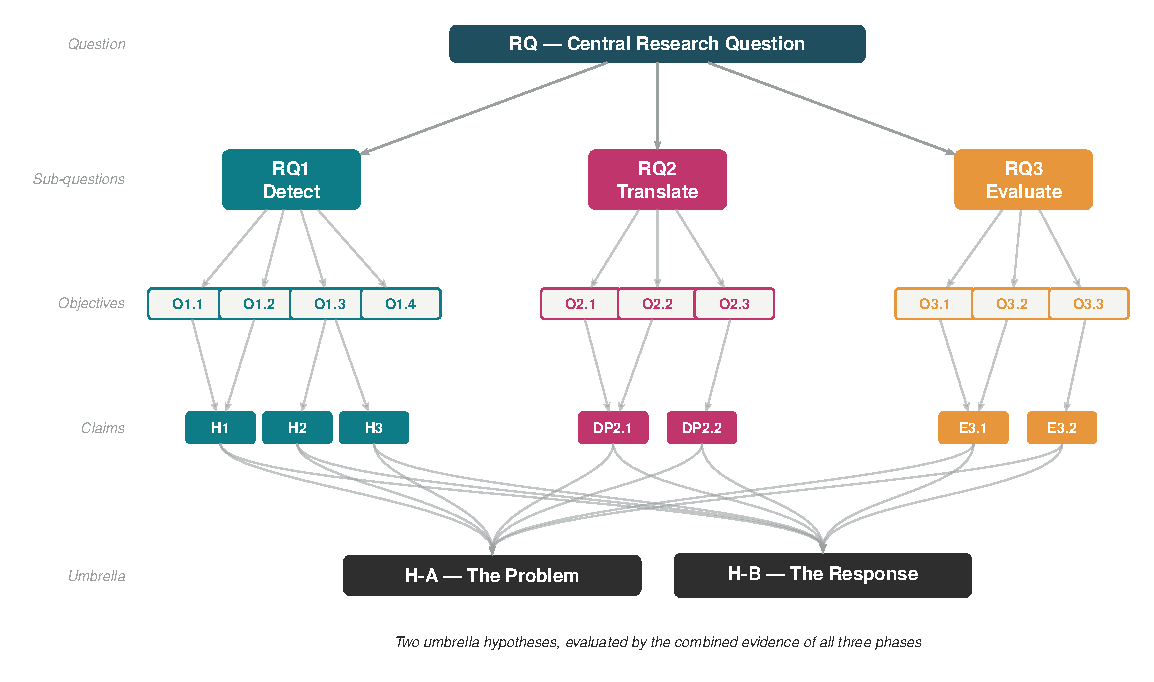
\includegraphics[width=\textwidth]{figures/research_questions/rq_tree_preview.pdf}
    \caption[Structure of the research questions, objectives, claims and umbrella hypotheses.]{\textbf{The
    architecture of the research programme.} The central research question branches into three
    sub-questions along the detect--translate--evaluate arc. Each sub-question generates its objectives
    (O1.1--O1.4, O2.1--O2.3, O3.1--O3.3), which give rise to the claims appropriate to their epistemic
    character: directional hypotheses (H1--H3), design propositions (DP2.1--DP2.2) and empirical
    expectations (E3.1--E3.2). All three claim groups converge on the two umbrella hypotheses, H-A (the
    problem) and H-B (the response), assessed not by any single instrument but by the combined evidence
    of the whole programme.}
    \label{fig:rq-tree}
\end{figure}
% =========================================================================

\begin{figure}[!ht]
    \centering
    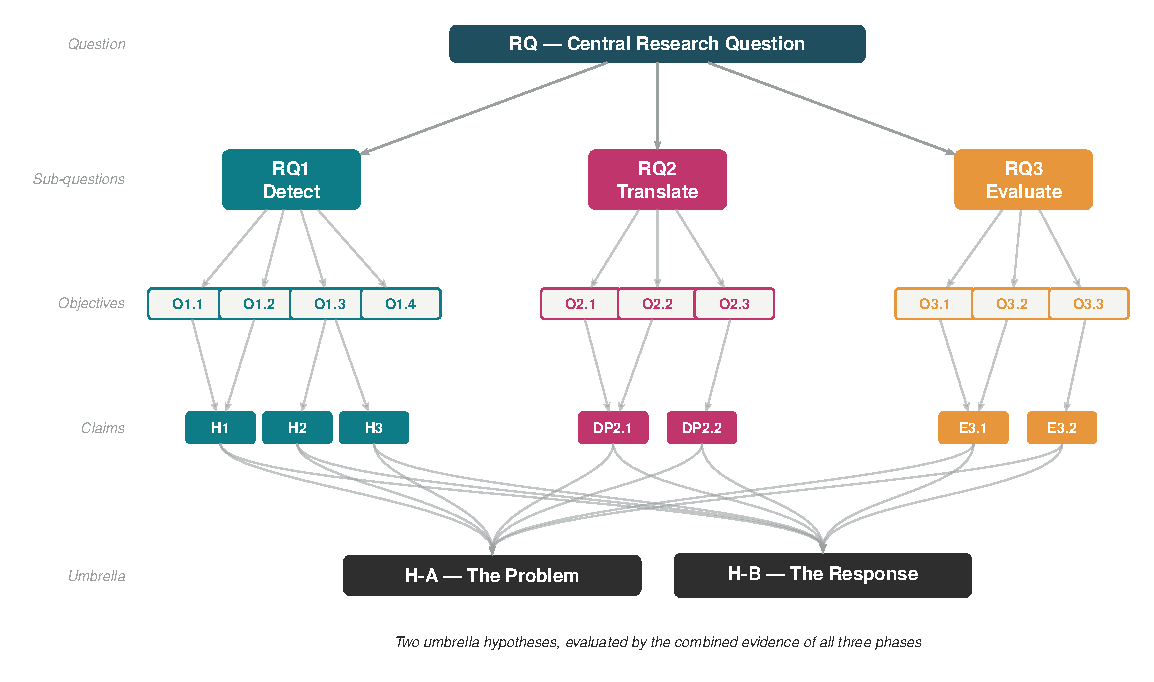
\includegraphics[width=\textwidth]{figures/research_questions/rq_tree_preview.pdf}
    \caption[Structure of the research questions, objectives, claims and umbrella hypotheses.]{\textbf{The
    architecture of the research programme.} The central research question branches into three
    sub-questions along the detect--translate--evaluate arc. Each sub-question generates its objectives
    (O1.1--O1.4, O2.1--O2.3, O3.1--O3.3), which give rise to the claims appropriate to their epistemic
    character: directional hypotheses (H1--H3), design propositions (DP2.1--DP2.2) and empirical
    expectations (E3.1--E3.2). All three claim groups converge on the two umbrella hypotheses, H-A (the
    problem) and H-B (the response), assessed not by any single instrument but by the combined evidence
    of the whole programme.}
    \label{fig:rq-tree}
\end{figure}